Selles peatükis analüüsime eelmises peatükis kirjeldatud katsete tulemusi, et mõista, kuidas erinevad mudelikonfiguratsioonid ja treeningstrateegiad mõjutavad metsastunud ja lageraielõikude tuvastamise täpsust satelliitpiltidelt. Arutatakse ka tulemuste statistilist olulisust ning võrreldakse erinevate lähenemiste efektiivsust.
\section{Tulemuste võrdlus}
\textbf{Baasjoon}

Eksperimendi käigus testiti süstemaatiliselt erinevaid hüperparameetreid, et leida optimaalne konfiguratsioon antud ülesande jaoks. 
Esitatud tulemuste (all\_metrics.json) analüüs näitas, et parimad mudelid
saavutasid märkimisväärselt kõrgeid Dice'i skoore, ulatudes kuni \textasciitilde
0.984. See on eriti üllatav, arvestades andmestiku väiksust.

Parimaks osutunud mudeli konfiguratsioon oli järgmine:
\begin{itemize}
  \item \textbf{Arhitektuur:} Unet
  \item \textbf{Enkooder:} ResNet50
  \item \textbf{Enkooderi kaalud:} ImageNet (eelkoolitatud)
  \item \textbf{Optimeerija:} AdamW
  \item \textbf{Õpisamm:} \textasciitilde 1.09e-4
\end{itemize}

Ka teised kombinatsioonid,
näiteks DeepLabV3 koos ResNet50-ga, saavutasid kõrgeid tulemusi (Dice > 0.97).
Osaliselt on tipptulemused visualiseeritud ka lisatud joonisel \ref{fig:segmentation_results}.

\textbf{Kõrgete skooride põhjused}
Kõrgeid tulemusi väikesel andmestikul võib seletada mitme teguriga.
Siirdõpe (\textit{Transfer Learning}): ImageNet andmestikul eelkoolitatud enkooderite
kasutamine on tõenäoliselt peamine edu võti. Eelnevalt treenitud mudelid omavad
juba võimekust tuvastada üldiseid visuaalseid mustreid (nt servad, tekstuurid),
mida saab efektiivselt kohandada spetsiifilisele metsanduse segmenteerimise
ülesandele. See vähendab oluliselt vajamineva treeningandmestiku mahtu. Peaaegu
kõik parimad tulemused saavutati just imagenet kaaludega. 
Ülesobitamise(\textit{Overfitting}) risk. Kuigi valideerimistulemused on kõrged, tuleb väikese
andmestiku puhul alati arvestada ülesobitamise ohuga. Samas näitab all\_metrics.
json faili analüüs, et paljudel juhtudel valideerimis- ja treeningkahju
(val\_loss, train\_loss) vähenesid sünkroonis, mis viitab sellele, et mudelid
suutsid siiski valideerimisandmetele edukalt üldistuda ega õppinud
treeningandmeid lihtsalt pähe.

\begin{figure}[H]
    \centering
    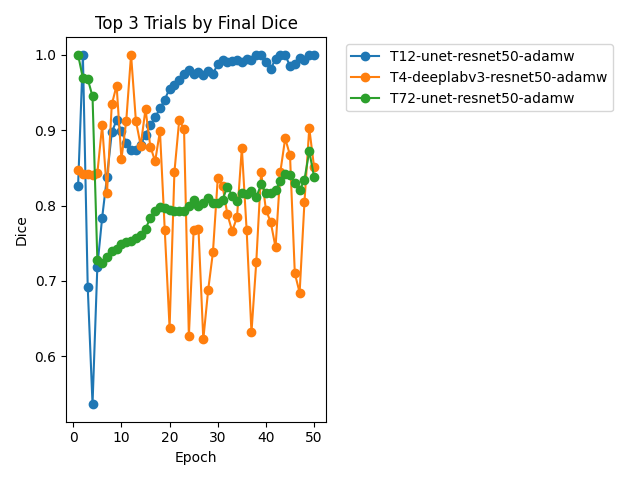
\includegraphics[width=0.8\textwidth]{figures/top3_dice.png}
    \caption{Parimad DICE tulemused erinevate mudelite vahel.}
    \label{fig:segmentation_results}
\end{figure}





\section{Edasiarendus ja täiustamine}
\input{chapters/edasiarendus_ja_täiustamine.tex}